%% %% 版本作者:
%% %%   Wizen Zhang
%% %%   E-mail:wizen_zhang@163.com
%% %%   GitHub:https://github.com/WizenZhang/NMUThesis
%% %%=================================================================
%% %% <UTF-8>
%% %% 北方民族大学学位论文LaTeX模板--始于 2018/08/02
%% %% 请将以下文件与此LaTeX文件放在同一目录中.
%% %%-----------
%% %% NMUThesis.tex         : LaTeX模板(main)
%% %% NMUThesis.pdf         : PDF模板样例
%% %% nmu.cls               : LaTeX宏模板文件
%% %% GBT7714-2005.bst      : 国标参考文献BibTeX样式文件2005(https://github.com/Haixing-Hu/GBT7714-2005-BibTeX-Style)
%% %% GBT7714-2015.bst      : 国标参考文献BibTeX样式文件2015(https://github.com/zepinglee/gbt7714-bibtex-style)
%% %% nmu_logo.png          : 论文封面北方民族大学校标
%% %% tex/*.tex             : LaTeX模板样例中的独立章节
%% %% figures/*             : LaTeX模板样例中的插图存放目录
%% %% ref.bib               : LaTeX模板中的参考文献Bib文件
%% %% make.bat              : 生成NMUThesis.pdf
%% %% clean.bat             : 清理冗余文件
%% %%-----------
%% %% 请统一使用UTF-8编码.
%% %%=================================================================
%% %%LaTeX安装配置教程请参看:https://jingyan.baidu.com/article/b2c186c83c9b40c46ff6ff4f.html
%% %%LaTeX入门视频教程请参看:https://blog.csdn.net/so_geili/article/details/51702564
%=================================================================
\documentclass[master,oneside,ultimate,MS]{nmu}
%=================================================================
% nmu基于ctexbook模板
% 论文样式参考自院教字〔2003〕169号《北方民族大学研究生学位论文格式和要求》
% 本模板改写自《北京航空航天大学学术论文LaTeX模板》
% 部分样例参考《浙江大学研究生硕士(博士)学位论文LaTeX模板》
%======================
% 模板选项:
% \documentclass[<thesis>,<printtype>,<version>,<subject>]{nmu}
%======================
% I.论文类型(thesis)
%--------------------
% a.学术硕士论文(master)<缺省值>
% b.专业硕士论文(professional)
% c.博士论文(doctor)
%--------------------
% II.打印属性(printtype)
%--------------------
% a.单面打印(onside)<缺省值>
% b.双面打印(twoside)
%--------------------
% III.论文版本(version)
%--------------------
% a.盲审版(blind)<缺省值>
% b.最终版(ultimate)
%--------------------
% IV.学科设置(subject)
%--------------------
% a.理工类(MS)<缺省值>
% b.文史类(MA)
%--------------------
%=================================================================

%=================================================================
% 开启/关闭引用编号颜色:参考文献,公式,图,表,算法 等……
\refcolor{off}   % 开启: on; 关闭: off<默认>;
% 摘要和正文从右侧开始
\beginright{on} % 开启: on<默认>; 关闭: off;
% 空白页
\emptypagewords{}

%=================================================================
% nmu模板已内嵌以下LaTeX工具包:
%--------------------
% ifthen, etoolbox, titletoc, remreset, remreset,
% geometry, fancyhdr, setspace, caption,
% float, graphicx, subfigure, epstopdf,
% booktabs, longtable, multirow, 
% array, enumitem
% algorithm2e, amsmath, amsthm, listings
% pifont, color, soul
%--------------------
% 请在此处添加额外工具包>> 


%=================================================================
% nmu模板已内嵌以下LaTeX宏:
%--------------------
% \highlight{text} % 黄色高亮
%--------------------
% 请在此处添加自定义宏>> 

%=================================================================
% 插图路径设置,图片放在figures 文件夹下。一般来说论文的插图比较多,通常按章节存
% 放,因此可以在以下命令中在按章节添加存放图片的文件夹路径。如以下这个路径中 ./
% 代表当前NMUThesis.tex所在的目录,就是一般所说的当前文件夹;figures 文件夹就是子文件
% 夹,存放正文及附录中要用到的所有的图片,在figures 文件夹中的子文件夹就是存放各
% 个章节图片的文件夹,一般命名与相应章节的名字相同,如chap_sample章节用到的图片全放在
% 了sample这个子文件夹下。
\graphicspath{{./figures/sample/},{./figures/}}
%%=================================================================
% 论文标题
\title{北方民族大学研究生学位论文\LaTeX{}模板\\ \NMUThesis{}}
% 根据ulem的文档第五页说明,通过宏或者命令传递到uline 命令中的英文句子是被盒子装
% 起来的,如果不特殊处理,则句子无法断行,但是\\,\ ,和 \- 还是可以起作用,因此
% 须在\englishtitle命令中的句子的适当位置添加"\",使句子可以断行。中文则不存在此
% 问题。 

\englishtitle{\LaTeX{} Template For The Academic Dissertaion Of North Minzu University}
\author{学生姓名}
% 分类号
\classification{TP227}
% 单位代码
\serialnumber{11407}
% 密级
\secretlevel{公开}
% 学号
\studentnumber{20160000}
% 指导教师(空格:~)
\supervisor{导师一教授~~导师二教授}
% 申请的学位门类
\applyclass{工学硕士}
% 专业名称
\major{计算机系统结构}
% 研究方向
\research{学位论文\LaTeX{}编程研究}
% 所在学院
\institute{计算机科学与工程学院}
% 提交日期
\submitdate{2019年3月}
% 毕业届(页眉)
\session{2019}
%%=================================================================
% 摘要-{中文}{英文}
\Abstract{%
摘要是学位论文极为重要、不可缺少的组成部分,它是论文的窗口,并频繁用于国内外资料交流、情报检索、二次文献编辑等。其性质和要求一般为:

1.摘要即摘录论文要点,是论文要点不加注释和评论的一篇完整的陈述性短文,具有很强的自含性和独立性,能独立使用和被引用。

2.摘要应含有学位论文全文的主要信息,一般包括研究目的、研究方法、所取得的结果和结论。论文摘要应突出新见解或创新性。

3.摘要的详简度视论文的内容、性质而定,硕士学位论文摘要一般为500$\sim$600字,但不能超过1000字。

4.摘要中一般不用图、表、化学结构式、计算机程序,不用非公知公用的符号、术语和非法定的计量单位。

5.“摘要” 居中用三号黑体字,3倍行间距;“关键词” 另起一行置于摘要下方,左对齐,用四号宋体加粗;摘要和关键词的内容用小四号宋体,行间距为1.5倍行距。

6.摘要一般为3至5个,中间以“,”分隔,涉及的内容、领域从大到小排列,便于文献编目与查询。

7.应有与中文摘要和关键词相对应的英文摘要和关键词。英文摘要用词要准确使用本学科通用词汇;摘要中主语(作者)常常省略,因而一般使用被动语态;应使用正确的时态并要注意主谓语的一致,必要的冠词不能省略。

8.英文摘要和关键词字号与中文一样,用Times New Roman字体;涉及到的姓名、书名等用斜体。

  }{%
  \LaTeX{} is a system for typesetting documents. It was originally created by Leslie Lamport and is now maintained by a group of volunteers {\it(http://latex-project.org)}. It is widely used, particularly for complex and technical documents, such as those involving mathematics.
  
  A \LaTeX{} user writes an input file containing text along with interspersed commands, for instance commands describing how the text should be formatted. It is implemented as a set of related commands that interface with Donald E. Knuth’s TeX typesetting program (the technical term is that \LaTeX{} is a macro package for the TeX engine). The user produces the output document by giving that input file to the TeX engine.
  
  The term \LaTeX{} is also sometimes used to mean the language in which the document is marked up, that is, to mean the set of commands available to a \LaTeX{} user.
  
  The name \LaTeX{} is short for “Lamport TeX”. It is pronounced LAH-teck or LAY-teck, or sometimes LAY-tecks. Inside a document, produce the logo with \LaTeX{}. Where use of the logo is not sensible, such as in plain text, write it as ‘\LaTeX{}’.
}
% 关键字-{中文}{英文}
\Keyword{%
    北民大,学位论文,博士,学硕,专硕,\LaTeX{}模板}{%
    NMUThesis,Dissertaion,Doctor,Master,Professional,\LaTeX{}Template
}

% 图标目录

\Listfigtab{off} % 启用: on<默认>; 关闭: off;

\begin{document}

%%=================================================================
% 标题级别
%--------------------
% \chapter{第一章}
% \section{1.1 小节}
% \subsection{1.1.1 条}
% \subsubsection{1.1.1.1}
% \paragraph{1.1.1.1.1}
% \subparagraph{1.1.1.1.1.1}
%--------------------
%%=================================================================
% 绪论
% [绪论]
% 此次为本LaTeX模板的简介
\chapter{绪论}
大家好,这是北方民族大学学术论文\LaTeX{}模板(\CTeX{}-Based)---\NMUThesis{}。

\NMUThesis{}为北民大研究生学术论文模板,适用于理工类学术硕士和专业硕士。本\LaTeX{}模板参考自院教字〔2003〕169号《北方民族大学研究生学位论文格式和要求》(以下简称《格式》),具体要求请参见《格式》,最终成文格式需参考学院要求及打印方意见。本模板中大量内容和说明直接摘抄自《格式》,基本覆盖了论文内容和格式方面的要求。

文献著录BibTeX样式采用Haixing Hu开源的2005版参考文献著录BibTeX样式\href{https://github.com/Haixing-Hu/GBT7714-2005-BibTeX-Style}{GBT7714-2005}及Zeping Lee开源的2015版参考文献著录BibTeX样式\href{https://github.com/zepinglee/gbt7714-bibtex-style}{GBT7714-2015},在此感谢两位的开源分享。请自行选用:\\
\verb|\bibliographystyle\{GBT7714-2005\}|或\\
\verb|\bibliographystyle\{GBT7714-2015\}|。

本模板改写自《北京航空航天大学学术论文LaTeX模板》,已上传至GitHub\footnote{\href{https://github.com/WizenZhang/NMUThesis}{https://github.com/WizenZhang/NMUThesis}}。

意见及问题反馈请联系:\\
\indent E-mail:wizen\_zhang@163.com\\
\indent GitHub:\href{https://github.com/WizenZhang/NMUThesis/issues}{https://github.com/WizenZhang/NMUThesis/issues}

%%============================
\section{概述}
硕士研究生学位论文是学位申请人为申请硕士学位而撰写的学术论文,它集中表明了作者在研究工作中获得的新成果,是评判学位申请人学术水平的重要依据和获得学位的必要条件之一,也是科研领域中的重要文献资料和社会的宝贵财富。为提高我校硕士学位论文的质量,规范学位论文格式,特作如下规定。

%%============================
\section{基本要求}

\begin{enumerate}[label=\arabic*)]
	\item 硕士学位论文应能表明作者确已在本门学科上掌握了坚实的基础理论和系统的专门知识,并对所研究课题有新的见解,有从事科学研究工作或独立担负专门技术工作的能力。
	
	\item 除外语专业外,学位论文一般用中文撰写,硕士学位论文正文应不少于2万字。学位论文内容应立论正确、推理严谨、文字简练、层次分明、说理透彻、数据真实可靠。
	
	\item 量和单位及其符号均应符合国家标准的规定,国家标准中未规定的,应执行国际标准或行业标准;不同的量必须用不同的符号表示,不得一符多义,含义相同的量则必须用同一符号表示。学位论文应用最新颁布的汉语简化文字,符合《出版物汉字使用管理规定》;专业术语应统一使用全国自然科学名词审定委员会公布的各学科名词,或本学科权威和期刊通用的专业术语,且前后应一致;标点符号的使用应符合国家标准《标点符号用法》的规定;数字的使用应符合国家标准《出版物上数字用法的规定》。
	
	\item 图要精选,切忌与文字或表内容重复,图中文字、数据和符号应准确无误且与文字叙述一致,图应有图名,图名应简洁明确且与图中内容相符。表应用表序和表名,表名应简洁并与内容相符。图、表和公式应分别顺序编号。
\end{enumerate}

论文内容包括:选题的背景、依据及意义;文献及相关研究综述、研究及设计方案、实验方法、装置和实验结果;理论的证明、分析和结论;重要的计算、数据、图表、曲线及相关分析;必要的附录、相关的参考文献目录等,如表\ref{tab:papercomponents}。

\centerline{-----------$\downarrow$-----------Space Check-----------$\downarrow$-----------}
\begin{table}[h]
  \caption{学术论文组成}
  \label{tab:papercomponents}
  \centering
  \begin{tabular}{cp{16\ccwd}p{4cm}}
    \toprule
    {\bfseries 装订顺序} & \multicolumn{1}{c} {\bfseries 内容} & \multicolumn{1}{c} {\bfseries 说明}  \\
    \midrule
    1 & 封面& \\
    3 & 独创性声明和使用授权书 & \\
    4 & 中文摘要        & \\
    5 & 英文摘要        & \\
    6 & 目录            & \\
    7 & 正文            & \\
    8 & 结论/结语	        & \\
    9 & 参考文献        & \\
    10& 附录            & 非必要 \\
    12& 致谢            & 盲审论文无此项 \\
    13& 个人简介        & 盲审论文无此项 \\
    \bottomrule
  \end{tabular}
\end{table}
\centerline{-----------$\uparrow$-----------Space Check-----------$\uparrow$-----------}
%%============================

\section{版式及其它要求}

%%============================

%%----------------------
\subsection{开本及版心}
{\bfseries 论文开本大小}:210mm×297mm(标准A4纸)。

{\bfseries 论文版心}:左边距:30mm,右边距:25mm,上边距:30mm,下边距:25mm,页眉边距:23mm,页脚边距:20mm。
%%----------------------
\subsection{页眉及页脚}

\begin{enumerate}[label=\arabic*)]
	\item 从正文开始各页均加有页眉、页脚,文字均采用小五号宋体。
	
	\item 页眉左侧为“北方民族大学×××届硕士学位论文”,右侧为一级标题名称;页眉下横线为上粗下细文武线(3磅)。
	
	\item 页码格式为“-1-”,单面打印时,插入的页码排在页脚居中的位置;双面打印时,插入的页码分别排在页脚左右侧。
	
	\item 从内封面到目录,均用英文页码,如“I、II、III”,从引言到论文末页,页码用阿拉伯数字,如“-1-、-2-、-3-”。
\end{enumerate}

%%----------------------
\subsection{封面}

\begin{enumerate}[label=\arabic*)]
	\item 论文内外封面内容一样,外封皮用草绿色暗纹纸。
	
	\item 论文题目中英文对照,均可分两行排列;中文用黑体二号字,英文用Times New Roman三号字。
	
	\item 分类号按《中国图书资料分类法》要求查询填写。
	
	\item 密级:涉密论文,学院学位评定分委员会根据国家规定的密级范围和法定程序审查确定,并注明相应的保密年限;不需保密的应填写“公开”。
	
	\item 论文完成日期统一用阿拉伯数字填写。
\end{enumerate}

%%----------------------

%%----------------------
\subsection{独创性声明和使用授权书}

独创性声明和关于论文使用授权的说明附于内封面后,需由研究生和指导教师本人签字。

%%----------------------
%%============================

\section{论文各组成部分要求}

%%============================
%%----------------------
\subsection{摘要及关键词}

\begin{enumerate}[label=\arabic*)]
	\item 摘要即摘录论文要点,是论文要点不加注释和评论的一篇完整的陈述性短文,具有很强的自含性和独立性,能独立使用和被引用。
	
	\item 摘要应含有学位论文全文的主要信息,一般包括研究目的、研究方法、所取得的结果和结论。论文摘要应突出新见解或创新性。
	
	\item 摘要的详简度视论文的内容、性质而定,硕士学位论文摘要一般为500-600字,但不能超过1000字。
	
	\item 摘要中一般不用图、表、化学结构式、计算机程序,不用非公知公用的符号、术语和非法定的计量单位。
	
	\item “摘要” 居中用三号黑体字,3倍行间距;“关键词” 另起一行置于摘要下方,左对齐,用四号宋体加粗;摘要和关键词的内容用小四号宋体,行间距为1.5倍行距。
	
	\item 摘要一般为3至5个,中间以“,”分隔,涉及的内容、领域从大到小排列,便于文献编目与查询。
	
	\item 应有与中文摘要和关键词相对应的英文摘要和关键词。英文摘要用词要准确使用本学科通用词汇;摘要中主语(作者)常常省略,因而一般使用被动语态;应使用正确的时态并要注意主谓语的一致,必要的冠词不能省略。
	
	\item 英文摘要和关键词字号与中文一样,用Times New Roman字体;涉及到的姓名、书名等用斜体。
\end{enumerate}

%%----------------------
\subsection{目录}

\begin{enumerate}[label=\arabic*)]
	\item 目录依论文内的章节标题次序排列,标题应该简明扼要。
	
	\item 目录中仅出现两级标题,文史类目录标题为第一章、第一节,理工类目录标题为第一章、1.1。
	
	\item “目录” 居中用黑体二号字,一级标题左对齐用宋体四号字,二级标题与一级标题左空一个字的位置,用宋体小四号字。

\end{enumerate}

%%----------------------
\subsection{正文}

\begin{enumerate}[label=\arabic*)]
	\item 正文是论文的主体,一般由标题、文字叙述、图、表和公式等五个部分构成。写作形式可因科研项目的性质不同而变化,一般可包括理论分析、计算方法、实验装置和测试方法,经过整理加工的实验结果分析和讲座,与理论计算结果的比较以及本研究方法与已有研究方法的比较等。
	
	\item 正文分章节撰写,每章都另起一页。
	
	\item 正文内容使用五号宋体字,行间距为1.5倍行距。
	
\end{enumerate}

%%----------------------
\subsection{标题}
\begin{enumerate}[label=\arabic*)]
	\item 论文标题是以最恰当、最简明的词语反映论文中最重要的特定内容的逻辑组合。标题既要准确地描述内容,又要尽可能地短,一级标题一般不宜超过36个字。标题应该避免使用不常见的缩略词、字符、代号和公式等。
	
	\item 论文标题一般分为三级,文史类与理工类标题格式不同,具体如下:
	
	{\bfseries 文史类}:
	
	第一章(一级标题,居中,黑体三号字,3倍行间距)
	
	第一节(二级标题,居中,黑体四号字,2.5倍行间距)
	
	一、(三级标题,首行缩进2字符,黑体小四号字,2倍行间距)
	如有四五六级标题,可按如下格式:
	
	(一)(四级标题,首行缩进2字符,宋体五号字,2倍行间距)
	1.(五级标题,首行缩进2字符,宋体五号字,2倍行间距)
	
	(1)(六级标题,首行缩进2字符,宋体五号字,2倍行间距)
	
	{\bfseries 理工类}:
	
	第一章(一级标题,居中,黑体三号字,3倍行间距)
	
	1.1(二级标题,左对齐,黑体四号字,2.5倍行间距)
	
	1.1.1(三级标题,左对齐,黑体小四号字,2倍行间距)
	
	\item “参考文献”、“附录”、“致谢”、“个人简介”等标题为居中黑体三号字,3倍行间距;内容使用宋体小四号字,1.5倍行间距。
	
\end{enumerate}

%%----------------------
\subsection{注释}

\begin{enumerate}[label=\arabic*)]
	\item 所有引用、参考、借用的资料数据及他人成果必须标明出处,严禁抄袭、剽窃。
	
	\item 引用文献标注方式应全文统一,文中引用内容使用上标标注,以 \textcircled{1}、\textcircled{2}等为编号标于所引内容最末句右上角,用小五号宋体字;解释内容采用脚注方式,以\textcircled{1}、\textcircled{2}为序号置于页下,用小五号宋体字,两端对齐,单倍行距。
	
	\item 不同页的脚注序号不需要连续编号;同一页几处引用同一文献时,将所有序号一起列出,只标注一次出处。
	
\end{enumerate}

%%----------------------
\subsection{参考文献}

\begin{enumerate}[label=\arabic*)]
	\item 参考文献采用尾注形式,标注于正文结束之后,不得罗列在各章节后。
	
	\item 引用文献标注方式应全文统一,文中引用内容使用上标标注,以 \textcircled{1}、\textcircled{2}等为编号标于所引内容最末句右上角,用小五号宋体字;解释内容采用脚注方式,以\textcircled{1}、\textcircled{2}为序号置于页下,用小五号宋体字,两端对齐,单倍行距。
	
	\item 各类文献资料的排列格式为:
	
	{\bfseries 期刊类}:
	[序号]作者.题目.刊名,出版年份,卷号(期号)
	
	{\bfseries 专(译)著类}:
	[序号]作者.书名(,译者).出版地:出版社,出版年,起止页码
	
	{\bfseries 论文集}:
	[序号]作者.题名,见(英文用In),主编,论文集名,出版地:出版社,出版年,起止页码
	
	{\bfseries 学位论文}:
	[序号]作者,题名,授予单位所在地:授予单位,授予年
	
	{\bfseries 专利}:
	[序号]申请者,专利名,国别,专利文献种类,专利号,出版日期
	
	{\bfseries 技术标准}:
	[序号]发布单位,标准代号,标准顺序号-发布年,标准名称,出版地,出版者,出版日期
	
	{\bfseries 电子文献}:
	[序号]作者.题名.获取或访问路径
	
\end{enumerate}

%%----------------------
\subsection{附录(非必要)}

\begin{enumerate}[label=\arabic*)]
	\item 主要列正文内容过于冗长的公式推导,供查读方便所需的辅助性数学工具或表格;重复性数据图表;论文使用缩写、程序全文及说明等。
	
	\item 附录编号顺序依次为附录1,附录2、附录3……,每个附录应有标题。
	
\end{enumerate}

%%----------------------
\subsection{致谢}

\begin{enumerate}[label=\arabic*)]
	\item 致谢对象仅限对完成课题研究和论文写作过程给予指导和帮助的导师、任课教师、校内外专家、实验技术人员、同学等。
	
	\item 致谢内容以精练的叙述性文字内容为主,用词应含蓄、笼统、简朴,不宜出现感情色彩浓厚和流于俗套的溢美之词,不宜出现图表等。
	
\end{enumerate}

%%----------------------
\subsection{个人简介}

\begin{enumerate}[label=\arabic*)]
	\item 简要介绍自己,内容包括姓名,性别,民族,籍贯,第一学历毕业院校及专业,取得的学位。
	
	\item 在研期间发表的论文,内容包括发表刊物名称,年月、卷册号,页码、论文作者排序及署名单位名称等,罗列论文以发表的时间先后排列。
	
\end{enumerate}

%%============================

\section{编排顺序及打印及装订等要求}

\begin{enumerate}[label=\arabic*)]
	\item 学位论文的编排顺序为外封面、内封面、独创性声明和授权说明、中文摘要、英文摘要、目录、引言/绪论、正文、结论/结语、注释和参考文献、附录、致谢、个人简介等部分。
	
	\item 学位论文内容一律用计算机编辑,用A4规格纸打印,按以上要求装订成册(不得用活页夹装订)。
\end{enumerate}

%%============================

% 示例
% 本LaTeX模板的使用示例
\chapter{示例}
\label{sec:sample}
%==============================
\section{参考文献引用}
参考文献类型:专著[M],会议论文集[C],报纸文章[N],期刊文章[J],学位论文[D],报告[R],标准[S],专利[P],论文集中的析出文献[A]。测试一下上标引用\upcite{Le2016Multiple},引用\cite{Le2016Multiple,Kaya2015,tf2017},还有其它引用\upcite{Li2017An,Le2016Multiple,tf2017}.
%--------------------------------
\subsection{数字标注}
\noindent
\begin{tabular}{l@{\quad$\Rightarrow$\quad}l}
	\verb|\cite{Li2017An}| & \cite{Li2017An}\\
	\verb|\citet{Li2017An}| & \citet{Li2017An}\\
	\verb|\citet[chap.~2]{Li2017An}| & \citet[chap.~2]{Li2017An}\\[0.5ex]
	\verb|\citep{Li2017An}| & \citep{Li2017An}\\
	\verb|\citep[chap.~2]{Li2017An}| & \citep[chap.~2]{Li2017An}\\
	\verb|\citep[see][]{Li2017An}| & \citep[see][]{Li2017An}\\
	\verb|\citep[see][chap.~2]{Li2017An}| & \citep[see][chap.~2]{Li2017An}\\[0.5ex]
	\verb|\citet*{Li2017An}| & \citet*{Li2017An}\\
	\verb|\citep*{Li2017An}| & \citep*{Li2017An}\\
\end{tabular}
\par\noindent
\begin{tabular}{l@{\quad$\Rightarrow$\quad}l}
	\verb|\citet{Li2017An,Kaya2015}| & \citet{Li2017An,Kaya2015}\\
	\verb|\citep{Li2017An,Kaya2015}| & \citep{Li2017An,Kaya2015}\\
	\verb|\cite{Li2017An,lamport1994}| & \cite{Li2017An,lamport1994}\\
	\verb|\upcite{Li2017An,lamport1994}| & \upcite{Li2017An,lamport1994}\\
	\verb|\citet{Li2017An,lamport1994}| & \citet{Li2017An,lamport1994}\\
	\verb|\citep{Li2017An,lamport1994}| & \citep{Li2017An,lamport1994}\\
	\verb|\cite{Li2017An,lamport1994,Kaya2015}| & \cite{Li2017An,lamport1994,Kaya2015}\\
\end{tabular}

%--------------------------------
\subsection{数字标注-上标形式}
\noindent
\begin{tabular}{l@{\quad$\Rightarrow$\quad}l}
	\verb|\upcite{Li2017An}| & \upcite{Li2017An}\\
	\verb|\upcite{Li2017An,lamport1994,Kaya2015}| & \upcite{Li2017An,lamport1994,Kaya2015}\\
\end{tabular}
\par\noindent
实现源码:\verb|\newcommand{\upcite}[1]{\textsuperscript{\cite{#1}}}|。


%--------------------------------
\subsection{著者-出版年制标}
\citestyle{authoryear}
\noindent
\begin{tabular}{l@{\quad$\Rightarrow$\quad}l}
	\verb|\cite{Li2017An}| & \cite{Li2017An}\\
	\verb|\citet{Li2017An}| & \citet{Li2017An}\\
	\verb|\citet[chap.~2]{Li2017An}| & \citet[chap.~2]{Li2017An}\\[0.5ex]
	\verb|\citep{Li2017An}| & \citep{Li2017An}\\
	\verb|\citep[chap.~2]{Li2017An}| & \citep[chap.~2]{Li2017An}\\
	\verb|\citep[see][]{Li2017An}| & \citep[see][]{Li2017An}\\
	\verb|\citep[see][chap.~2]{Li2017An}| & \citep[see][chap.~2]{Li2017An}\\[0.5ex]
	\verb|\citet*{Li2017An}| & \citet*{Li2017An}\\
	\verb|\citep*{Li2017An}| & \citep*{Li2017An}\\
\end{tabular}
\par\noindent
\begin{tabular}{l@{\quad$\Rightarrow$\quad}l}
	\verb|\citet{Li2017An,Kaya2015}| & \citet{Li2017An,Kaya2015}\\
	\verb|\citep{Li2017An,Kaya2015}| & \citep{Li2017An,Kaya2015}\\
	\verb|\cite{Li2017An,lamport1994}| & \cite{Li2017An,lamport1994}\\
	\verb|\citet{Li2017An,lamport1994}| & \citet{Li2017An,lamport1994}\\
	\verb|\citep{Li2017An,lamport1994}| & \citep{Li2017An,lamport1994}\\
\end{tabular}
\citestyle{numbers}

%--------------------------------
\subsection{其他形式的标注}
\noindent
\begin{tabular}{l@{\quad$\Rightarrow$\quad}l}
	\verb|\citealt{Kaya2015}| & \citealt{Kaya2015}\\
	\verb|\citealt*{Kaya2015}| & \citealt*{Kaya2015}\\
	\verb|\citealp{Kaya2015}| & \citealp{Kaya2015}\\
	\verb|\citealp*{Kaya2015}| & \citealp*{Kaya2015}\\
	\verb|\citealp{Kaya2015,Li2017An}| & \citealp{Kaya2015,Li2017An}\\
	\verb|\citealp[pg.~32]{Kaya2015}| & \citealp[pg.~32]{Kaya2015}\\
	\verb|\citenum{Kaya2015}| & \citenum{Kaya2015}\\
	\verb|\citetext{priv.\ comm.}| & \citetext{priv.\ comm.}\\
\end{tabular}

\noindent
\begin{tabular}{l@{\quad$\Rightarrow$\quad}l}
	\verb|\citeauthor{Kaya2015}| & \citeauthor{Kaya2015}\\
	\verb|\citeauthor*{Kaya2015}| & \citeauthor*{Kaya2015}\\
	\verb|\citeyear{Kaya2015}| & \citeyear{Kaya2015}\\
	\verb|\citeyearpar{Kaya2015}| & \citeyearpar{Kaya2015}\\
\end{tabular}

\section{浮动体\footnote{样例参考《浙江大学研究生硕士(博士)学位论文\LaTeX{}模板》}}
在实际撰写文稿的过程中,我们可能会碰到一些占据篇幅较大,但同时又不方便分页的内容。(比如图片和表格,通常属于这样的类型)此时,我们通常会希望将它们放在别的地方,避免页面空间不够而强行置入这些内容导致 overfull vbox 或者大片的空白。此外,因为被放在别的地方,所以,我们通常需要对这些内容做一个简单的描述,确保读者在看到这些大块的内容时,不至于无从下手去理解。同时,因为此类内容被放在别的地方,所以在文中引述它们时,我们无法用「下图」、「上表」之类的相对位置来引述他们。于是,我们需要对它们进行编号,方便在文中引用。

在 \LaTeX{} 中,默认有 figure 和 table 两种浮动体。(当然,你还可以自定义其他类型的浮动体)在这些环境中,可以用 $\backslash$caption\{\} 命令生成上述简短的描述。至于编号,也是用 $\backslash$caption\{\} 生成的。这类编号遵循了 TeX 对于编号处理的传统:它们会自动编号,不需要用户操心具体的编号数值。 至于「别的地方」是哪里,\LaTeX{} 为浮动体启用了所谓「位置描述符」的标记。基本来说,包含以下几种:

h - 表示 here。此类浮动体称为文中的浮动体(in-text floats)。

t - 表示 top。此类浮动体会尝试放在一页的顶部。

b - 表示 bottom。此类浮动体会尝试放在一页的底部。

p - 表示 float page,浮动页。此类浮动体会尝试单独成页。

\LaTeX{} 会将浮动体与文本流分离,而后按照位置描述符,根据相应的算法插入 \LaTeX{} 认为合适的位置。

\subsection{插图测试}
如图\ref{fig:first_image_tset}是对此模版的第一张插图测试。
\begin{figure}[htb]
	\centering
	
\includegraphics[width = 5cm]{Chapter1.png}
	\caption{第一张插图测试}\label{fig:first_image_tset}
\end{figure}
以下是一段对这些插图来历的介绍,引用自知乎专栏All about TeXnique中夏晓昊的文章\href{http://zhuanlan.zhihu.com/LaTeX/19669122}{《The TeXbook导读:从那头(多图杀猫的)狮子说起》}。

在The TeXbook中,有着一系列的以狮子为主题的插图。这些插图的作者是Duane Bibby。也是从The TeXbook开始,不少TeX书也采取了以狮子为主的插图,作者也是Duane Bibby。另外,每年的TUG(TeX Users Group)年会都会有一张以狮子为主题的logo,这只狮子已经是社区的吉祥物了。

为什么选择狮子呢?Yannis Haralambous写道(原文法语,此为转译后的英文):Not for nothing is TeX represented by a lion. Donald Knuth has told us that lions are to him the guardians of libraries in the United States because there is a statue of a lion in front of the entrance of each large library there. Guardian of libraries, guardian of the Book—is that not indeed what TeX ultimately aspires to be? 或许吧。 (顺便说一句,TeX和MetaFont都用了狮子,TeX是公狮子,MetaFont是母狮子,多么和谐的一对啊。如果你还是忽略MetaFont的存在,那你还没有认识到它的重要性。)

作为插图,首要的一点就是贴切,然后是有趣。在TeX社区里面,have fun是一个很重要的词组,也有人说Happy TeXing。我知道有不少人不喜欢TeX,但是能有什么理由呢?如果你用不到它,那么浅尝辄止即可。如果你会用到很频繁,最好慢慢修炼做到精通。如果你只是偶尔用到,那么可以搬个模版什么的,甚至也可以找人帮你(不要指望别人会用足够的空闲时间来帮你,他没有这个义务,请支付报酬,最少也得请吃个饭吧)。下面的插图,是TeX TeXbook中的,我也希望这个假期,能有人有空来看看这本书。即使不能把所有的东西都看懂,那么也会对TeX的设计有了一定的了解,拿到扳手就好。

\subsection{表格测试}
在这里推荐制表采用功能强大的tabu宏包以取代其它制表宏包。具体tabu宏包的使用说明参见tabu宏包的说明文档。

以下节分别用来测试各种表格环境如,tabular,tabu,longtabu等,还有对caption格式的修改和测试。以下表格样式全部采用三线表。

\subsection{array宏包tabular表格环境测试}
如表\ref{tab:first_table_test}是对array宏包的tabular表格环境测试。

\begin{table}[htb]
	\centering
	\caption{tabular环境的编程语言优缺点对比表格}\label{tab:first_table_test}
	\begin{tabular}{lrr}
		\toprule
		\textbf{编程语言}     & \textbf{优势} & \textbf{劣势} \\
		\midrule
		Python     & 简单易学  & 速度较慢 \\
		C/C++     & 跨平台性能好    & 学习难度大 \\
		Java     & 使用范围最广 & 占用内存大 \\
		\bottomrule
	\end{tabular}%
\end{table}

\subsection{tabu宏包表格环境测试}
如表\ref{tab:tabu_test_1}是对tabu宏包的tabu表格环境测试。在这里表格命令与表\ref{tab:first_table_test}的命令相同,只是tabular环境改成了tabu环境。
\begin{table}[htb]
	\centering
	\caption{tabu环境的编程语言优缺点对比表格}\label{tab:tabu_test_1}
	\begin{tabu}{lrr}
		\toprule
		\textbf{编程语言}     & \textbf{优势} & \textbf{劣势} \\
		\midrule
		C$\#$     & 全面集成.Net库  & 跨平台能力太差 \\
		JavaScript     & 学习难度低    & 过于依赖浏览器 \\
		SQL    & 开发速度快,安全性好 & 运行速度换开发速度 \\
		\bottomrule
	\end{tabu}%
\end{table}

表\ref{tab:tabu_test_2}对tabu to表格的x列模式进行测试。在表格导言区中设置为X[1]X[2]X[2],表示这三列表格的列宽比值为1:2:2,总的表格宽度由tabu to环境设置,这里设置为0.6\textbackslash linewidth。相比于tabular环境,tabu环境的列宽设置方便许多。
\begin{table}[htb]
	\centering
	\caption{tabu环境的编程语言优缺点对比表格---X列模式}\label{tab:tabu_test_2}
	\begin{tabu} to 0.6\linewidth{X[1]X[2]X[2]}
		\toprule
		\textbf{编程语言}     & \textbf{优势} & \textbf{劣势} \\
		\midrule
		PHP     & 社区庞大活跃易上手  & 运行速度慢 \\
		Kotlin     & 和Java互操作性佳    & 继承了Java劣势 \\
		Swift     & 在iOS占比变大 & 版本更迭快差异大 \\
		\bottomrule
	\end{tabu}%
\end{table}

如表\ref{tab:tabu_test_3}是longtabu环境测试表格。longtabu环境不能用在table浮动体环境中。根据GB/T 7713.1-2006规定:如果某个表需要转页接排,在随后的各页上应重复表的编号。编号后跟标题(可省略)和“(续)”,置于表上方。续表应重复表头。

特别需要注意的是,longtabu是基于longtable宏包开发的,所以在nmu.cls文件中已经插入了longtable宏包。longtable环境的所有功能都可以在longtabu中使用,如\textbackslash endhead,\textbackslash endfirsthead,\textbackslash endfoot,\textbackslash endlastfoot,和\textbackslash caption等。具体用法请参见longtable和tabu宏包的相应文档。

在 9 月份的 TIOBE 编程语言排行榜中,Python 超越 C++,首次进入排行榜 TOP 3。事实上,无论在工业界还是学术界,Python 的使用者越来越多,尤其是近年来 —— 乃至可以预见的未来,在 AI和数据分析这些热门的领域,Python 都将会有大展拳脚的天地。所以反映在 TIOBE 排行榜上就是逐渐上升的排名。

不过在最新的 10 月编程语言排行榜中如表\ref{tab:tabu_test_3},刚被挤下 TOP 3 的 C++ 反超 Python,以 0.44$\%$ 的微弱优势重新夺回第三的宝座。毕竟 C++ 在服务端、游戏开发和实时体系等应用范畴中,早已有庞大的使用者,而且诞生的时间也比 Python 早。所以未来的排行榜中,我们相信 C++ 和 Python 应该会处于“反超与被反超”这样一种交替超越的状态。
\begin{longtabu}{cccccc}
	\caption{2018年10月全球编程语言TIOBE排行榜}\label{tab:tabu_test_3}\\
	\toprule
	Oct-18	&	Oct-17	&	Change	&	Programming Language	&	Ratings	&	Change	\\
	\midrule%
	\endfirsthead
	\caption{2018年10月全球编程语言TIOBE排行榜(续)}\\
	\toprule
	Oct-18	&	Oct-17	&	Change	&	Programming Language	&	Ratings	&	Change	\\
	\midrule%
	\endhead
	\bottomrule%
	\endfoot
	1	&	1	&		&	Java	&	17.801$\%$	&	5.37$\%$	\\
	2	&	2	&		&	C	&	15.376$\%$	&	7$\%$	\\
	3	&	3	&		&	C++	&	7.593$\%$	&	2.59$\%$	\\
	4	&	5	&	$\uparrow$	&	Python	&	7.156$\%$	&	3.35$\%$	\\
	5	&	8	&	$\uparrow$	&	Visual Basic .NET	&	5.884$\%$	&	3.15$\%$	\\
	6	&	4	&	$\downarrow$	&	C$\#$	&	3.485$\%$	&	-0.37$\%$	\\
	7	&	7	&		&	PHP	&	2.794$\%$	&	0$\%$	\\
	8	&	6	&	$\downarrow$	&	JavaScript	&	2.28$\%$	&	-0.73$\%$	\\
	9	&	-	&	$\uparrow$	&	SQL	&	2.038$\%$	&	2.04$\%$	\\
	10	&	16	&	$\uparrow$	&	Swift	&	1.5$\%$	&	-0.17$\%$	\\
	11	&	13	&	$\uparrow$	&	MATLAB	&	1.317$\%$	&	-0.56$\%$	\\
	12	&	20	&	$\uparrow$	&	Go	&	1.253$\%$	&	-0.1$\%$	\\
	13	&	9	&		&	Assembly language	&	1.245$\%$	&	-1.13$\%$	\\
	14	&	15	&	$\uparrow$	&	R	&	1.214$\%$	&	-0.47$\%$	\\
	15	&	17	&	$\uparrow$	&	Objective-C	&	1.202$\%$	&	-0.31$\%$	\\
	16	&	12	&	$\downarrow$	&	Perl	&	1.168$\%$	&	-0.8$\%$	\\
	17	&	11	&	$\downarrow$	&	Delphi/Object Pascal	&	1.154$\%$	&	-1.03$\%$	\\
	18	&	10	&	$\downarrow$	&	Ruby	&	1.108$\%$	&	-1.22$\%$	\\
	19	&	19	&		&	PL/SQL	&	0.779$\%$	&	-0.63$\%$	\\
	20	&	18	&	$\downarrow$	&	Visual Basic	&	0.652$\%$	&	-0.77$\%$	\\
	21	&		&		&	D	&	0.643$\%$	&		\\
	22	&		&		&	SAS	&	0.609$\%$	&		\\
	23	&		&		&	Dart	&	0.543$\%$	&		\\
	24	&		&		&	Scratch	&	0.496$\%$	&		\\
	25	&		&		&	COBOL	&	0.478$\%$	&		\\
	26	&		&		&	Scala	&	0.454$\%$	&		\\
	27	&		&		&	F$\#$	&	0.438$\%$	&		\\
	28	&		&		&	Groovy	&	0.435$\%$	&		\\
	29	&		&		&	Lua	&	0.405$\%$	&		\\
	30	&		&		&	ABAP	&	0.396$\%$	&		\\
\end{longtabu}

另外值得关注的还有 Swift,按照 TIOBE 的说法,“Swift 正在敲开 TIOBE 排行榜前 10 名的大门”。根据观察,排行榜中 TOP 9 的编程语言已基本稳定,唯独第 10 名每个月都会有变化。在本月中,Swift 的排名就上升到了第 10 的位置,且试图成为 TIOBE TOP 10 的固定成员。与此同时,Ruby 和 Perl 也正在争夺这个位置。不过 TIOBE 认为,按照此前的趋势来看,目前编程语言 TOP 10 的候选人似乎有 3 位:Swift、Go 和 R,但它们也并不一定能够成功站稳,原因如下:

\begin{itemize}
	\item Swift 显然是开发 iOS 移动应用程序的头号编程语言。但由于它仅适用于 iOS 而不适用于 Android,因此程序员更多的是选择采用“一次编写到处运行”的框架。
	\item 编程语言 R 正在受到新贵 Python 的碾压性竞争。
	\item Go 语言,与其他编程语言相比,并没有过于亮眼的优点,所以还不清楚是什么让它脱颖而出。
\end{itemize}

话虽如此,但我们依然有理由相信,Go 依然是一只优质的“潜力股”,且不说它一直保持上升的趋势,在日益火热的云服务领域,Go 语言基本上已是事实上的“龙头”地位。

需要注意的是,SQL 自 2018 年 2 月起被重新添加到了TIOBE排行榜中,由于没有以往的数据可以对比,所以会给人 SQL 语言指数突然暴涨的错觉,历史排名如表\ref{tab:tabu_test_4}所示。

\begin{longtabu}{lccccccc}
	\caption{历史排名(1988-2018/每5年)}\label{tab:tabu_test_4}\\
	\toprule
	Programming Language	&	2018	&	2013	&	2008	&	2003	&	1998	&	1993	&	1988	\\	
	\midrule%
	\endfirsthead
	\caption{历史排名(1988-2018/每5年)(续)}\\
	\toprule
	Programming Language	&	2018	&	2013	&	2008	&	2003	&	1998	&	1993	&	1988	\\
	\midrule%
	\endhead
	\bottomrule%
	\endfoot
	Java	&	1	&	2	&	1	&	1	&	17	&	-	&	-	\\
	C	&	2	&	1	&	2	&	2	&	1	&	1	&	1	\\
	C++	&	3	&	4	&	3	&	3	&	2	&	2	&	4	\\
	Python	&	4	&	7	&	6	&	11	&	24	&	13	&	-	\\
	C$\#$	&	5	&	5	&	7	&	8	&	-	&	-	&	-	\\
	Visual Basic .NET	&	6	&	11	&	-	&	-	&	-	&	-	&	-	\\
	PHP	&	7	&	6	&	4	&	5	&	-	&	-	&	-	\\
	JavaScript	&	8	&	9	&	8	&	7	&	21	&	-	&	-	\\
	Ruby	&	9	&	10	&	9	&	18	&	-	&	-	&	-	\\
	R	&	10	&	23	&	48	&	-	&	-	&	-	&	-	\\
	Objective-C	&	14	&	3	&	40	&	50	&	-	&	-	&	-	\\
	Perl	&	16	&	8	&	5	&	4	&	3	&	9	&	22	\\
	Ada	&	29	&	19	&	18	&	15	&	12	&	5	&	3	\\
	Lisp	&	30	&	12	&	16	&	13	&	8	&	6	&	2	\\
	Fortran	&	31	&	24	&	21	&	12	&	6	&	3	&	15	\\
\end{longtabu}
TIOBE 编程社区指数(The TIOBE Programming Community index)是编程语言流行度的指标,该榜单每月更新一次,指数基于全球技术工程师、课程和第三方供应商的数量。包括流行的搜索引擎,如谷歌、必应、雅虎、维基百科、亚马逊、YouTube 和百度都用于指数计算。具体的计算方式见这里:\href{https://www.tiobe.com/tiobe-index/programming-languages-definition/}{https://www.tiobe.com/tiobe-index/programming-languages-definition/}。

值得注意的是,TIOBE 指数并不代表语言的好坏,开发者可以使用该榜单检查自身的编程技能是否需要更新,或者在开始构建新软件时对某一语言做出选择。
\subsection{子图}
这里子图的排版推荐使用subcaption宏包,不再推荐使用subfig宏包,更不推荐使用subfigure宏包。值得注意的是,在nmu.cls文件中已经写入了subcaption宏包,而且subcaption宏包与subfigure和subfig宏包是相互冲突的。因此,如果你还想使用subfig宏包而不想使用subcaption宏包,请自己到nmu.cls文件的相关位置更改,具体的使用及修改方法参见相应的宏包说明文档。不过在这里还是不推荐直接去更改nmu.cls文档,除非你对\LaTeX{} 的相关命令很清楚,知道自己在改什么,并且不会对其他格式产生影响。

具体的subcaption宏包使用方法我这里不仔细介绍,以下只是对subcaption进行一些简单的测试,主要是格式调整和交叉引用。

如图\ref{fig:subfig_test1}是有两张子图的模式,对子图进行交叉引用,如图\ref{subfig:1a}和图\ref{subfig:1b}。

\begin{figure}[htbp]
	\centering
	\begin{subfigure}[b]{.4\textwidth}
		\centering
		
\includegraphics[width = \textwidth]{Chapter2.png}
		\caption{书籍排版与普通排版}\label{subfig:1a}
	\end{subfigure}
	\quad
	\begin{subfigure}[b]{.4\textwidth}
		\centering
		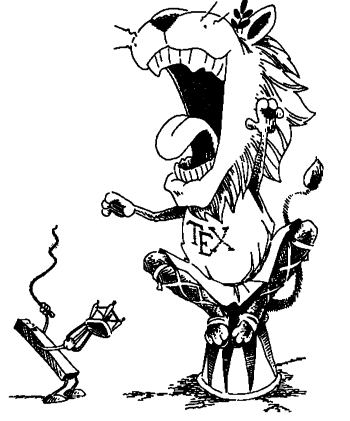
\includegraphics[width = \textwidth]{Chapter3.png}
		\caption{\TeX 的控制系列}\label{subfig:1b}
	\end{subfigure}
	\caption{子图模式测试1:2张图}\label{fig:subfig_test1}
\end{figure}

如图\ref{fig:subfig_test2}是有四张子图的模式,对子图进行交叉引用,如图\ref{subfig:2a}、图\ref{subfig:2b}、图\ref{subfig:2c}和图\ref{subfig:2d}。

\begin{figure}[htbp]
	\centering
	\begin{subfigure}[b]{.4\textwidth}
		\centering
		
\includegraphics[width = \textwidth]{Chapter4.png}
		\caption{字体}\label{subfig:2a}
	\end{subfigure}
	\begin{subfigure}[b]{.4\textwidth}
		\centering
		
\includegraphics[width = \textwidth]{Chapter5.png}
		\caption{编组}\label{subfig:2b}
	\end{subfigure}
	\begin{subfigure}[b]{.4\textwidth}
		\centering
		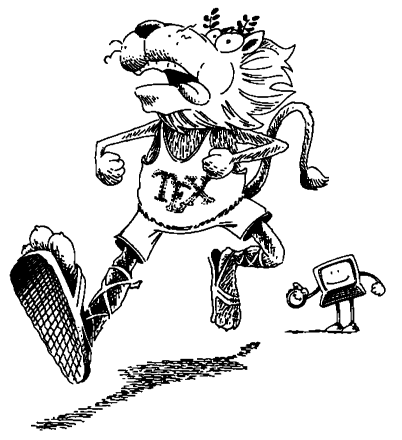
\includegraphics[width = \textwidth]{Chapter6.png}
		\caption{运行\TeX}\label{subfig:2c}
	\end{subfigure}
	\begin{subfigure}[b]{.4\textwidth}
		\centering
		
\includegraphics[width = \textwidth]{Chapter7.png}
		\caption{\TeX 工作原理}\label{subfig:2d}
	\end{subfigure}
	\caption{子图模式测试2:4张图}\label{fig:subfig_test2}
\end{figure}

\section{算法环境}

模板中使用 \texttt{algorithm2e} 宏包实现算法 \ref{alg:partition},关于该宏包的具体用法请阅读宏包的官方文档。

\begin{algorithm}[!h]
	%\SetAlgoLined
	%\SetAlgoVlined
	\caption{A How to (plain).}
	\KwData{this text}
	\KwResult{how to write algorithm with \LaTeX2e{} }
	
	initialization\;
	\While{not at end of this document}{
		read current\;
		\eIf{understand}{
			go to next section\;
			current section becomes this one\;
		}{
			go back to the beginning of current section\;
		}
	}
\end{algorithm}

\RestyleAlgo{ruled}
\begin{algorithm}[!h]
	\caption{A How to (ruled).}
	\KwData{this text}
	\KwResult{how to write algorithm with \LaTeX2e{} }
	
	initialization\;
	\While{not at end of this document}{
		read current\;
		\eIf{understand}{
			go to next section\;
			current section becomes this one\;
		}{
			go back to the beginning of current section\;
		}
	}
\end{algorithm}


\RestyleAlgo{boxed}
\begin{algorithm}[!h]
	\caption{A How to (boxed).}
	\KwData{this text}
	\KwResult{how to write algorithm with \LaTeX2e{} }
	
	initialization\;
	\While{not at end of this document}{
		read current\;
		\eIf{understand}{
			go to next section\;
			current section becomes this one\;
		}{
			go back to the beginning of current section\;
		}
	}
\end{algorithm}

\RestyleAlgo{boxruled}
\begin{algorithm}[!h]
	\caption{PARTITION$(A,p,r)$ (boxruled)}%算法标题
	\label{alg:partition}
	\KwData{this text}
	\KwResult{how to write algorithm with \LaTeX2e{} }
	\begin{algorithmic}[1]%一行一个标行号
		\STATE $i=p$
		\FOR{$j=p$ to $r$}
		\IF{$A[j]<=0$}
		\STATE $swap(A[i],A[j])$
		\STATE $i=i+1$
		\ENDIF
		\ENDFOR
	\end{algorithmic}
\end{algorithm}

\section{代码环境}
\subsection{全局设置}
listings 是专用于代码排版的\LaTeX{}宏包,可对关键词、注释和字符串等使用不同的字体和颜色或颜色,也可以为代码添加边框、背景等风格。很多时候需要对文档中的代码进行解释,只有带有行号的代码才可以让解释更清晰,因为你只需要说第 x行代码有什么作用即可。如果没有行号,那对读者而言就太残忍了,他们不得不从你的文字叙述中得知行号信息,然后去一行一行的查到相应代码行。listings 宏包通过参数 numbers 来设定行号,该参数的值有两个,分别是 left 与right,表示行号显示在代码的左侧还是右侧。下面给出一份用于排版C语言程序代码样例如图\ref{fig:code}所示。
\begin{figure}[htb!]
	\centering
	\begin{lstlisting}[language={[ANSI]C}] 
int main(int argc, char ** argv) 
{ 
    /*格式化并输出结果到标准输出*/
    printf("`我爱TeXing`! \n"); 
    return 0; 
} 
	\end{lstlisting} 
	\caption{C语言程序代码样例}
	\label{fig:code}
\end{figure}

\subsection{显示中文}
listings 宏包默认是不支持包含中文字串的代码显示的,但是可以使用 “逃逸” 字串来显示中文。

在 \verb|\lstset| 命令中设置逃逸字串的开始符号与终止符号,推荐使用的符号是左引号,即 “ `”。

\section{流程图}

\subsection{流程图概述}

流程图是流经一个系统的信息流、观点流或部件流的图形代表。在企业中,流程图主要用来说明某一过程。这种过程既可以是生产线上的工艺流程,也可以是完成一项任务必需的管理过程。流程图是揭示和掌握封闭系统运动状况的有效方式。作为诊断工具,它能够辅助决策制定,让管理者清楚地知道,问题可能出在什么地方,从而确定出可供选择的行动方案。

流程图是表达算法思想最为有效的图形工具。作为计算机专业的学生,我们经常需要在文档中使用流程图来描述算法。在 LaTeX 中使用流程图可以通过 TikZ 或 flowchart 宏包来实现,但从本质上来说 flowchart 宏包也是使用 TikZ 宏包来实现的。flowchart 定义的形状数量比较少,可能满足不了绘制复杂流程图的需要,直接使用TikZ强大的绘图功能来实现流程图的绘制如图\ref{fig:chart},。

\begin{figure}[htb!]
	\centering
	\begin{tikzpicture}[node distance=1.8cm]
	%定义流程图具体形状
	\node (start) [startstop] {Start};
	\node (in1) [io, below of=start] {Input};
	\node (pro1) [process, below of=in1] {Process 1};
	\node (dec1) [decision, below of=pro1, yshift=-0.5cm] {Decision 1};
	\node (dec2) [decision, below of=dec1, yshift=-1.5cm] {Decision 2};
	\node (pro2) [process, right of=dec1, xshift=3cm] {Process 2};
	\node (out1) [io, below of=dec2, yshift=-0.5cm] {Output};
	\node (stop) [startstop, below of=out1] {Stop};
	\coordinate (pointN) at (-3cm, -9.2cm);
	%连接具体形状
	\draw [arrow](start) -- (in1);
	\draw [arrow](in1) -- (pro1);
	\draw [arrow](pro1) -- (dec1);
	\draw [arrow](dec1) -- (dec2);
	\draw [arrow](dec1) -- (pro2);
	\draw [arrow](dec1) -- node[anchor=east] {Y} (dec2);
	\draw [arrow](dec1) -- node[anchor=south] {N} (pro2);
	\draw [arrow](pro2) |- (pro1);
	\draw [arrow](dec2) -- node[left] {Y} (out1);
	\draw (dec2) -- node[above] {N} (pointN);
	\draw [arrow](pointN) |- (pro1);
	\draw [arrow](out1) -- (stop);
	\end{tikzpicture}
	\caption{直接使用TikZ宏包绘制的流程图}
	\label{fig:chart}
\end{figure}

\subsection{流程图的形式}
流程图常用的形式有两种:
 
(1)上下流程图 

上下流程图是最常见的一种流程图,它仅表示上一步与下一步的顺序关系。
 
(2)矩阵流程图

矩阵流程图不仅表示下下关系,还可以看出某一过程的其他关系。最后给一个流程图的例子如图\ref{fig:flowsheet}。流程图的原图来自于Itti的显著性论文。里面基本包含了常用流程图画法中的所有要点。

\subsection{\LaTeX{}中插入VISIO图}

1. VISIO原图另存为PDF格式

2. 用Acrobat打开,文档 -- 剪裁页面 -- 删除白边距

3. 将pdf格式文件复制到figures文件夹(盲审封皮文字:\verb|\includegraphics\{nmu-blind.pdf\}|)

4. 或另存为eps格式

5. 将eps格式文件复制到figures文件夹

6. 类似插入图片的方式将图插入

\begin{figure}[htb!]
	\centering
	%定义形状样式
	\tikzstyle{startstop} = [rectangle, rounded corners, minimum width = 3cm, minimum height = 0.7cm, text centered, draw = black]
	\tikzstyle{startstop2} = [rectangle, rounded corners, minimum width = 13cm, minimum height = 0.7cm, text centered, draw = black]
	\tikzstyle{io} = [trapezium, trapezium left angle = 30, trapezium right angle = 150, minimum width = 3cm, text centered, draw = black, fill = white]
	\tikzstyle{io2} = [trapezium, trapezium left angle = 30, trapezium right angle = 150, minimum width = 2.5cm, draw = black, fill = white]
	\tikzstyle{io3} = [trapezium, trapezium left angle = 30, trapezium right angle = 150, minimum width = 2cm, draw = black, fill = white]
	\tikzstyle{process} = [rectangle, minimum width = 3cm, minimum height = 1cm, text centered, draw = black]
	\tikzstyle{decision} = [diamond, minimum width = 3cm, minimum height = 1cm, text centered, draw = black]
	\tikzstyle{arrow} = [thick, -, >= stealth]
	\tikzstyle{arrow2} = [thick, ->, >= stealth]
	
	\begin{tikzpicture}[node distance = 1.5cm]
	% 定义流程图具体形状
	\coordinate[label = left:{\small 输入图像}](A) at(-1.5, 0);
	\node(in1) [io] {};
	\node(pro1) [startstop, below of = in1] {\small 线性滤波};
	
	\node(in2 - 2)[io3, below of = pro1, yshift = -0.6cm]{};
	\node(in3 - 2)[io3, left of = in2 - 2, xshift = -2.5cm]{};
	\node(in4 - 2)[io3, right of = in2 - 2, xshift = 2.5cm]{};
	
	\node(in2 - 1)[io2, below of = pro1, yshift = -0.3cm]{};
	\node(in3 - 1)[io2, left of = in2 - 1, xshift = -2.5cm]{};
	\node(in4 - 1)[io2, right of = in2 - 1, xshift = 2.5cm]{};
	
	\node(in2) [io, below of = pro1] {\small 颜色};
	\node(in3)[io, left of = in2, xshift = -2.5cm]{ \small 亮度 };
	\node(in4)[io, right of = in2, xshift = 2.5cm]{ \small 方向 };
	
	\node(in5)[startstop2, below of = in2 - 2]{ \small Center - Surround差异计算及归一化 };
	
	\node(in6 - 2)[io3, below of = in5, yshift = -0.6cm]{};
	\node(in7 - 2)[io3, left of = in6 - 2, xshift = -2.5cm]{};
	\node(in8 - 2)[io3, right of = in6 - 2, xshift = 2.5cm]{};
	
	\node(in6 - 1)[io2, below of = in5, yshift = -0.3cm]{};
	\node(in7 - 1)[io2, left of = in6 - 1, xshift = -2.5cm]{};
	\node(in8 - 1)[io2, right of = in6 - 1, xshift = 2.5cm]{};
	
	\node(in6) [io, below of = in5] {};
	\node(in7)[io, left of = in6, xshift = -2.5cm]{};
	\node(in8)[io, right of = in6, xshift = 2.5cm]{};
	
	\coordinate[label = left:{\small 特征图}](B) at(-1, -6.2);
	\coordinate[label = left:{\small (12张)}](C) at(-1.5, -7.5);
	\coordinate[label = left:{\small (6张)}](D) at(2.7, -7.5);
	\coordinate[label = left:{\small (24张)}](E) at(6.7, -7.5);
	
	\node(in9)[startstop2, below of = in6 - 2]{ \small 跨尺度合并及归一化 };
	
	\node(in10) [io, below of = in9] {};
	\node(in11)[io, left of = in10, xshift = -2.5cm]{};
	\node(in12)[io, right of = in10, xshift = 2.5cm]{};
	
	\coordinate[label = left:{\small 醒目图}](F) at(-1, -9.5);
	\node(in13) [startstop, below of = in10] {\small 线性组合};
	\node(in14) [io, below of = in13] {};
	\coordinate[label = left:{\small 显著图}](G) at(-1, -13);
	
	\node(in15) [startstop, below of = in14] {\small 赢者取全};
	\coordinate[label = left:{\small 显著位置}]() at(1, -16.1);
	\coordinate[label = left:{\small 反馈抑制}]() at(4.5, -14.7);
	
	%连线
	\draw[arrow](pro1) -- (in1);
	\draw[arrow](pro1) -- (in2);
	\draw[arrow](pro1) -- (in3);
	\draw[arrow](pro1) -- (in4);
	\draw[arrow](0, -4.75) -- (in2 - 2);
	\draw[arrow](-4, -4.75) -- (in3 - 2);
	\draw[arrow](4, -4.75) -- (in4 - 2);
	\draw[arrow](0, -5.45) -- (in6);
	\draw[arrow](-4, -5.45) -- (in7);
	\draw[arrow](4, -5.45) -- (in8);
	\draw[arrow](0, -8.35) -- (in6 - 2);
	\draw[arrow](-4, -8.35) -- (in7 - 2);
	\draw[arrow](4, -8.35) -- (in8 - 2);
	\draw[arrow](0, -9.05) -- (in10);
	\draw[arrow](-4, -9.05) -- (in11);
	\draw[arrow](4, -9.05) -- (in12);
	\draw[arrow](in13) -- (in10);
	\draw[arrow](in13) -- (in11);
	\draw[arrow](in13) -- (in12);
	\draw[arrow](in13) -- (in14);
	\draw[arrow](in14) -- (in15);
	\draw[arrow](in15) -- (0, -15.8);
	\draw[arrow](0, -15.4) -- (2.5, -15.4);
	\draw[arrow](2.5, -14) -- (2.5, -15.4);
	\draw[arrow2](2.5, -14) -- (0, -14);
	\end{tikzpicture}
	\caption{图形图像处理模型流程图}
	\label{fig:flowsheet}
\end{figure}

\section{数学环境}

\subsection{数学符号}

模板定义了一些正体(upright)的数学符号:
\begin{center}
	\begin{tabular}{rl}
		\toprule
		符号                 & 命令 \\
		\midrule
		常数$\eu$     & \verb|\eu| \\
		复数单位$\iu$ & \verb|\iu| \\
		微分符号$\diff$ & \verb|\diff| \\
		$\argmax$         & \verb|\argmax| \\
		$\argmin$         & \verb|\argmin| \\
		\bottomrule
	\end{tabular}
\end{center}

更多的例子:
\begin{equation}
\eu^{\iu\pi} + 1 = 0
\end{equation}
\begin{equation}
\frac{\diff^2u}{\diff t^2} = \int f(x) \diff x
\end{equation}
\begin{equation}
\argmin_x f(x)
\end{equation}

\subsection{定理、引理和证明}

\begin{definition}
	A sigmoid function is a mathematical function having a characteristic "S"-shaped curve or sigmoid curve. Often, sigmoid function refers to the special case of the logistic function shown in the first figure and defined by the formula:
	\begin{equation}
	sigmoid(x) = \frac{1}{1 + e^{-x}}
	\end{equation}
	
	\begin{figure}[htb]
		\centering
		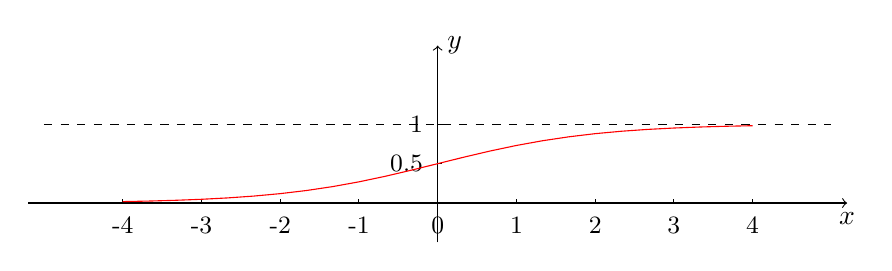
\begin{tikzpicture}
		\draw[->](-5.2,0)--(5.2,0)node[left,below]{$x$};
		\draw[->](0,-0.5)--(0,2)node[right]{$y$};
		\draw[dashed](-5,1)--(5,1);
		\foreach \x in {-4,-3,-2,-1,0,1,2,3,4}{\draw(\x,0)--(\x,0.05)node[below,outer sep=2pt,font=\small]at(\x,0){\x};}
		\foreach \y in {0.5,1}{\draw(0,\y)--(0.05,\y)node[left,outer sep=2pt,font=\small]at(0,\y){\y};}
		\draw[color=red ,domain=-4:4]plot(\x,{1/(1+(e^(-1*(\x))))});
		\end{tikzpicture}
	\end{figure}

	Special cases of the sigmoid function include the Gompertz curve (used in modeling systems that saturate at large values of x) and the ogee curve (used in the spillway of some dams). Sigmoid functions have domain of all real numbers, with return value monotonically increasing most often from 0 to 1 or alternatively from −1 to 1, depending on convention.
\end{definition}



\begin{example}
	Simple examples of functions on $\mathbf{R}^d$ that are integrable
	(or non-integrable) are given by
	\begin{equation}
	f_a(x) =
	\begin{cases}
	|x|^{-a} & \text{if } |x| \leq 1,\\
	0 & \text{if } x > 1.
	\end{cases}
	\end{equation}
	\begin{equation}
	F_a(x) = \frac{1}{1 + |x|^a}, \qquad \text{all } x \in \mathbf{R}^d.
	\end{equation}
	Then $f_a$ is integrable exactly when $a < d$, while $F_a$ is integrable
	exactly when $a > d$.
\end{example}

\begin{lemma}[Fatou]
	Suppose $\{f_n\}$ is a sequence of measurable functions with $f_n \geq 0$.
	If $\lim_{n \to \infty} f_n(x) = f(x)$ for a.e. $x$, then
	\begin{equation}
	\int f \leq \liminf_{n \to \infty} \int f_n.
	\end{equation}
\end{lemma}

\begin{remark}
	We do not exclude the cases $\int f = \infty$,
	or $\liminf_{n \to \infty} f_n = \infty$.
\end{remark}

\begin{corollary}
	Suppose $f$ is a non-negative measurable function, and $\{f_n\}$ a sequence
	of non-negative measurable functions with
	$f_n(x) \leq f(x)$ and $f_n(x) \to f(x)$ for almost every $x$. Then
	\begin{equation}
	\lim_{n \to \infty} \int f_n = \int f.
	\end{equation}
\end{corollary}

\begin{proposition}
	Suppose $f$ is integrable on $\mathbf{R}^d$. Then for every $\epsilon > 0$:
	\begin{enumerate}
		\renewcommand{\theenumi}{\roman{enumi}}
		\item There exists a set of finite measure $B$ (a ball, for example) such that
		\begin{equation}
		\int_{B^c} |f| < \epsilon.
		\end{equation}
		\item There is a $\delta > 0$ such that
		\begin{equation}
		\int_E |f| < \epsilon \qquad \text{whenever } m(E) < \delta.
		\end{equation}
	\end{enumerate}
\end{proposition}

\begin{theorem}
	Suppose $\{f_n\}$ is a sequence of measurable functions such that
	$f_n(x) \to f(x)$ a.e. $x$, as $n$ tends to infinity.
	If $|f_n(x)| \leq g(x)$, where $g$ is integrable, then
	\begin{equation}
	\int |f_n - f| \to 0 \qquad \text{as } n \to \infty,
	\end{equation}
	and consequently
	\begin{equation}
	\int f_n \to \int f \qquad \text{as } n \to \infty.
	\end{equation}
\end{theorem}

\begin{proof}
	Trivial.
\end{proof}


\subsection{自定义}

\newtheorem*{axiomofchoice}{Axiom of choice}
\begin{axiomofchoice}
	Suppose $E$ is a set and ${E_\alpha}$ is a collection of
	non-empty subsets of $E$. Then there is a function $\alpha
	\mapsto x_\alpha$ (a ``choice function'') such that
	\begin{equation}
	x_\alpha \in E_\alpha,\qquad \text{for all }\alpha.
	\end{equation}
\end{axiomofchoice}

\newtheorem{observation}{Observation}[chapter]
\begin{observation}
	Suppose a partially ordered set $P$ has the property
	that every chain has an upper bound in $P$. Then the
	set $P$ contains at least one maximal element.
\end{observation}
\begin{proof}[A concise proof]
	Obvious.
\end{proof}

\newtheorem{observationvar2}[observation]{Observationvar2}
\begin{observationvar2}
	Suppose a partially ordered set $P$ has the property
	that every chain has an upper bound in $P$. Then the
	set $P$ contains at least one maximal element.
\end{observationvar2}
\begin{proof}[A concise proof]
	Obvious.
\end{proof}


% 说明
% 本LaTeX模板的一般使用说明
\chapter{说明\footnote{章标题中脚注命令测试}}
\label{sec:instruction}

%-----------------------------
\section{宏包\footnote{节标题中脚注命令测试}使用}

请将表\ref{tab:tabu_file}中文件清单放在同一目录中,使用\LaTeX{}可以选择TexLive+TeXstudio的方式,安装教程可参看百度经验\footnote{\href{https://jingyan.baidu.com/article/b2c186c83c9b40c46ff6ff4f.html}{安装教程请参看 : https://jingyan.baidu.com/article/b2c186c83c9b40c46ff6ff4f.html}}。

\begin{longtable}{|c|>{\raggedright\arraybackslash}p{8cm}|}
	\caption{北方民族大学学位论文\LaTeX{}模板清单表}\label{tab:tabu_file}
	\endfirsthead
	\caption{北方民族大学学位论文\LaTeX{}模板清单表(续)}
	\endhead
	\hline 
	\rule[0ex]{0pt}{2.5ex} \verb|NMUThesis.tex| & $\triangleright$\LaTeX{}模板运行入口(main) \\ 
	\hline 
	\rule[0ex]{0pt}{2.5ex} \verb|NMUThesis.pdf| & $\triangleright$PDF模板样例\\
	\hline 
	\rule[0ex]{0pt}{2.5ex} \verb|nmu.cls |    & $\triangleright$ \LaTeX{}宏模板文件 \\
	\hline 
	\rule[0ex]{0pt}{2.5ex} \verb|GBT7714-2005.bst| & $\triangleright$ 国标参考文献BibTeX样式文件2005 \\
	\hline 
	\rule[0ex]{0pt}{2.5ex} \verb|GBT7714-2015.bst|  & $\triangleright$ 国标参考文献BibTeX样式文件2015 \\
	\hline 
	\rule[0ex]{0pt}{2.5ex} \verb|nmu_logo.png|   & $\triangleright$论文封面北方民族大学校标 \\
	\hline 
	\rule[0ex]{0pt}{2.5ex} \verb|tex/*.tex| & $\triangleright$\LaTeX{}模板样例中的独立章节\\
	\hline 
	\rule[0ex]{0pt}{2.5ex} \verb|figures/*| & $\triangleright$\LaTeX{}模板样例中的插图存放目录\\
	\hline 
	\rule[0ex]{0pt}{2.5ex} \verb|ref.bib |    & $\triangleright$\LaTeX{}模板中的参考文献Bib文件\\
	\hline 
	\rule[0ex]{0pt}{2.5ex} \verb|make.bat|    &$\triangleright$生成NMUThesis.pdf\\
	\hline 
	\rule[0ex]{0pt}{2.5ex} \verb|clean.bat|  & $\triangleright$清理冗余文件\\
	\hline 
\end{longtable}

通过 \verb|\documentclass[<thesis>,<printtype>,<version>,<subject>]{nmu}|载入宏包,可选参数说明如下:
\begin{itemize}[leftmargin=3cm]
  \item[{\tt thesis} $\triangleright$]  论文类型(thesis),可选值:\\
    a) 学术硕士论文(\verb|master|)[缺省值]\hfill
    b) 专业硕士论文(\verb|professional|)\\
    c) 博士论文(\verb|doctor|)
  \item[{\tt printtype} $\triangleright$] 打印属性(printtype),可选值: \\
    a) 单面打印(\verb|onside|)[缺省值]\hfill
    b) 双面打印(\verb|twoside|)
  \item[{\tt version} $\triangleright$] 论文版本(version),可选值: \\
    a) 盲审版(\verb|blind|)[缺省值]\hfill
    b) 最终版(\verb|ultimate|)
  \item[{\tt subject} $\triangleright$] 学科设置(subject),可选值: \\
    a) 理工类(\verb|MS|)[缺省值]\hfill
    b) 文史类(\verb|MA|)
\end{itemize}

模板已内嵌\LaTeX{}工具包:
 {\tt ifthen},{\tt etoolbox},{\tt titletoc},{\tt remreset},{\tt remreset},
 {\tt geometry},{\tt fancyhdr},{\tt setspace},{\tt caption},{\tt float},
 {\tt graphicx},{\tt subfigure},{\tt epstopdf},
 {\tt book\-tabs},{\tt longtable},{\tt multirow},{\tt array}, {\tt enumitem},
 {\tt algorithm2e},{\tt amsmath},{\tt amsthm}, {\tt listings},
 {\tt pifont},{\tt color},{\tt soul}。

模板已内嵌宏:\verb|\highlight{text}|(黄色高亮)。
 
请统一使用UTF-8编码。

%-----------------------------
\section{章节撰写}
本模板支持一下标题级别标题级别

\begin{tabular}{ll}
  \verb|\chapter{章}|              & $\triangleright$ 第一章 \\
  \verb|\chapter*{无章号章}|       & $\triangleright$ 无章号章 \\
  \verb|\chaptera{无章有目录章}|   & $\triangleright$ 无章有目录章 \\
  \verb|\summary|                  & $\triangleright$ 总结\\
  \verb|\appendix|                 & $\triangleright$ 附录\\
  \verb|\acknowledgments|          & $\triangleright$ 致谢\\
  \verb|\biography|                & $\triangleright$ 个人简介\\
  \verb|\section{节}|              & $\triangleright$ 理工类:1.1 节 ~~~~文史类: 第一节 \\
  \verb|\subsection{条}|           & $\triangleright$ 理工类:1.1.1 条 ~~~~文史类:一、\\
  \verb|\subsubsection{A}|         & $\triangleright$ 理工类:1.1.1.1 A  ~~~~文史类: (一) ~~A\\
  \verb|\paragraph{a}|             & $\triangleright$ 理工类:1.1.1.1.1 a  ~~~~文史类: 1. ~~a\\
  \verb|\subparagraph{a)}|         & $\triangleright$ 理工类:1.1.1.1.1.1 a)  ~~~~文史类: (1) ~~a)\\
\end{tabular}

%-----------------------------
\section{选项设置}

\begin{itemize}[leftmargin=3cm]
	\item[{\tt  $\backslash$refcolor} $\triangleright$]  开启/关闭引用编号颜色,包括参考文献,公式,图,表,算法等\\
	\texttt{on}:开启 [默认]\\
	\texttt{off}:关闭
	\item[{\tt $\backslash$beginright} $\triangleright$]  摘要和正文从右侧开始\\
	\texttt{on}:开启 [默认]\\
	\texttt{off}:关闭
	\item[{\tt $\backslash$emptypageword} $\triangleright$]  空白页留字
	\item[{\tt $\backslash$Listfigtab} $\triangleright$]  是否使用图标清单目录\\
	\texttt{on}:开启 [默认]\\
	\texttt{off}:关闭
\end{itemize}


%-----------------------------
\section{注意事项}
\begin{itemize}
  \item[$\triangleright$] 暂无中文斜体;
  \item[$\triangleright$] 中文粗体将转换为楷体;
  \item[$\triangleright$] 目录中仅出现两级标题,通过\verb|\setcounter{tocdepth}{1}|设置两级标题目录深度;
  \item[$\triangleright$] 若某文献标题中含有特定含义大写字母(“ISODATA”等,详见\cite{Li2017An}),应特别用第二重{}将其括起来才可使其正常表示;
  \item[$\triangleright$] 切换论文版本后,重新生成目录需两次编译;
  \item[$\triangleright$] 行末针对标点的断行不好,例如\ref{sec:error1}处的有个“、”被断在了句首;
  \item[$\triangleright$] \verb|\label{<text>}|中不能使用中文;
  \item[$\triangleright$] 浮动体与正文之间的距离是弹性的;
  \item[$\triangleright$] 命令符与汉字之间请注意加空格以避免undefined错误(pdfLaTeX下好像一般不存在这个问题,主要在XeLaTeX编译环境下发生);
\end{itemize}

%-----------------------------
\section{ToDo}
\begin{itemize}
  \item[$\triangleright$] 模板选项参数选择(例:\verb|\documentclass[master,oneside,ultimate,MS]{nmu}|);
  \item[$\triangleright$] 导入BibTeX参考文献库可通过百度学术或Zotero等(例:如图\ref{fig:3-1}、\ref{fig:3-2});
  \item[$\triangleright$] 表格、图片可使用TeXstudio向导插入(例:如图\ref{subfig:3a}、\ref{subfig:3b});
\end{itemize}

\begin{figure}[tbh!]
	\centering
	
\includegraphics[width=0.6\linewidth]{figures/sample/3-1}
	\caption{导入BibTeX参考文献库步骤一}
	\label{fig:3-1}
\end{figure}

\begin{figure}[tbh!]
	\centering
	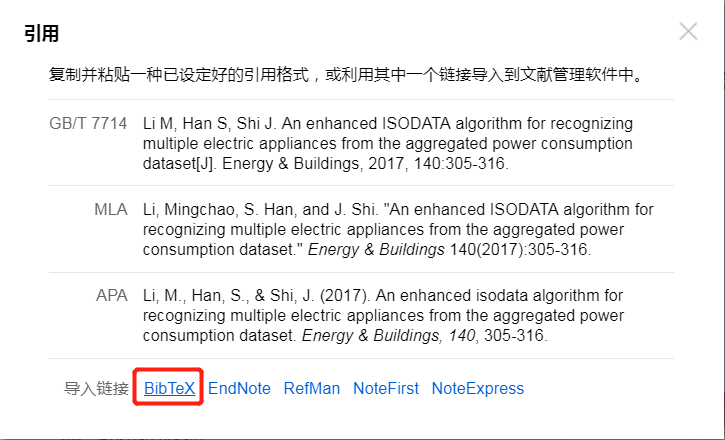
\includegraphics[width=0.6\linewidth]{figures/sample/3-2}
	\caption{导入BibTeX参考文献库步骤二}
	\label{fig:3-2}
\end{figure}

\begin{figure}[htb!]
	\centering
	\begin{subfigure}[b]{.4\textwidth}
		\centering
		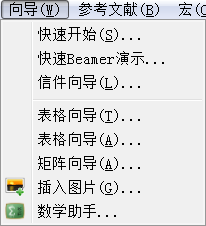
\includegraphics[width=0.7\linewidth]{3-3.png}
		\caption{TeXstudio向导}\label{subfig:3a}
	\end{subfigure}
	\begin{subfigure}[b]{.4\textwidth}
		\centering
		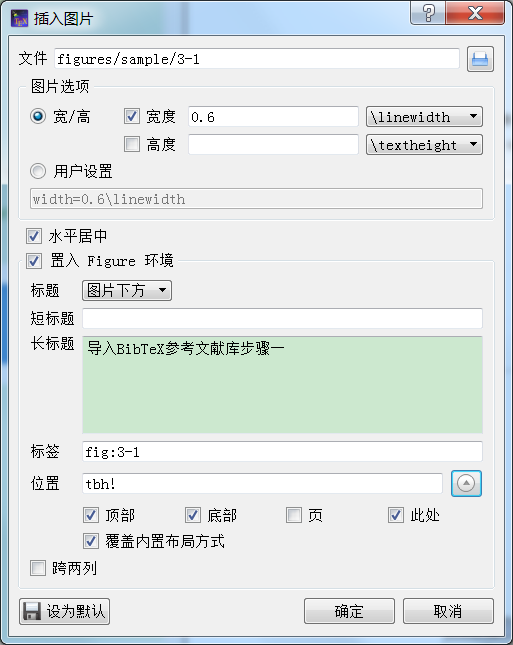
\includegraphics[width=\linewidth]{3-4.png}
		\caption{插入图片}\label{subfig:3b}
	\end{subfigure}
	\caption{使用TeXstudio向导插入图片}\label{fig:3}
\end{figure}
%-----------------------------
\section{意见及问题反馈}

\indent E-mail:wizen\_zhang@163.com\\
\indent GitHub:\href{https://github.com/WizenZhang/NMUThesis/issues}{https://github.com/WizenZhang/NMUThesis/issues}




% 总结
% 总结
\summary
%%%%%%%%%%%%%%%%%%%%%%%%%%%%%%%%%%%%%%%%%%%%%%%%%%%%%%%%
% 内容由此开始

学位论文的结论单独作为一章,但不加章号。如果不可能导出应有的结论,也可以没有结论而进行必要的讨论。

\begin{enumerate}[label=\arabic*)]
	\item 结论是对论文主要研究结果、论点的提炼与概括,主要阐述自己的创造性工作及所取得的研究成果在本学科学术领域中的地位、作用、意义、及本文研究的不足之处或未予解决的遗留问题。
	
	\item 结论要准确、完整、明确、精炼,对自己研究的评价要实事求是;要严格区分自己取得的成果与导师及他人的科研成果的界限。
\end{enumerate}

\par * 嗯,这就是你的论文了 * \par

% 内容到结束		
%%%%%%%%%%%%%%%%%%%%%%%%%%%%%%%%%%%%%%%%%%%%%%%%%%%%%%%%
\ifthenelse{\equal{\@beginright}{off}}{\clearpage}{\clearautopage}

% 参考文献
% [参考文献]
% \reference = \chapter{参考文献}
% 2015版国标GBT7714-2015
% 2005版国标GBT7714-2005
\reference
\xiaosi
\bibliographystyle{GBT7714-2015}
\bibliography{ref}
\thispagestyle{fancy}%添加页眉页脚


% 附录
% [附录]
% !!\acknowledgments =\= \chapter{附录}!!
% 不可替换使用\chapter{附录}
\appendix
\thispagestyle{fancy}%添加页眉页脚
\begin{enumerate}[label=\arabic*)]
\item 主要列正文内容过于冗长的公式推导,供查读方便所需的辅助性数学工具或表格;重复性数据图表;论文使用缩写、程序全文及说明等。

\item 附录编号顺序依次为附录1,附录2、附录3……,每个附录应有标题。
\end{enumerate}
下列内容可以作为附录:

\begin{enumerate}[label=\arabic*)]
\item 为了整篇论文材料的完整,但编入正文又有损于编排的条理和逻辑性,这一材料包括比正文更为详尽的信息、研究方法和技术更深入的叙述,建议可以阅读的参考文献题录,对了解正文内容有用的补充信息等;
\item 由于篇幅过大或取材于复制品而不便于编入正文的材料;
\item 不便于编入正文的罕见的珍贵或需要特别保密的技术细节和详细方案(这中情况可单列成册);
\item 对一般读者并非必要阅读,但对专业同行有参考价值的资料;
\item 某些重要的原始数据、过长的数学推导、计算程序、框图、结构图、注释、统计表、计算机打印输出文件等。
\end{enumerate}

\par * 嗯,自由发挥吧 * \par

% 致谢(盲审版不显示)
% [致谢]
\acknowledgments
\ifthenelse{\equal{\Show{}}{\show{}}}{% 是否显示[致谢]章
\begin{spacing}{1.3}\xiaosi %致谢内容为小四号
%%%%%%%%%%%%%%%%%%%%%%%%%%%%%%%%%%%%%%%%%%%%%%%%%%%%%%%%
% 内容由此开始

致谢中主要感谢指导教师和在学术方面对论文的完成有直接贡献及重要帮助的团体和人士,以及感谢给予转载和引用权的资料、图片、文献、研究思想和设想的所有者。致谢中还可以感谢提供研究经费及实验装置的基金会或企业等单位和人士。致谢辞应谦虚诚恳,实事求是,切记浮夸与庸俗之词。

\begin{enumerate}[label=\arabic*)]
	\item 致谢对象仅限对完成课题研究和论文写作过程给予指导和帮助的导师、任课教师、校内外专家、实验技术人员、同学等。
	\item 致谢内容以精练的叙述性文字内容为主,用词应含蓄、笼统、简朴,不宜出现感情色彩浓厚和流于俗套的溢美之词,不宜出现图表等。
\end{enumerate}

\par * 嗯,感谢完所有人之后,也请记得感谢一下自己 * \par
\vspace{18em}
\parbox[t][1cm][b]{\textwidth}{\hspace{20em}{
		签名:\par}}
	
\parbox[t][1cm][b]{\textwidth}{\hspace{23em}{
			\hspace{3em}年\hspace{2em}月\hspace{2em}日}}
		
% 内容到结束		
%%%%%%%%%%%%%%%%%%%%%%%%%%%%%%%%%%%%%%%%%%%%%%%%%%%%%%%%
\end{spacing}		
}{}

% 个人简介(盲审版不显示)
% [个人简介]
% \biography = \chapter{个人简介}
\biography
\ifthenelse{\equal{\Show{}}{\show{}}}{% 是否显示[个人简介]章
\begin{spacing}{1.3}\xiaosi %致谢内容为小四号
%%%%%%%%%%%%%%%%%%%%%%%%%%%%%%%%%%%%%%%%%%%%%%%%%%%%%%%%
% 内容由此开始

{\noindent \bfseries 基本信息:}

简要介绍自己,内容包括姓名,性别,民族,籍贯,第一学历毕业院校及专业,取得的学位,现阶段就读院校及专业。

{\noindent \bfseries 在研期间发表的论文:}

\begin{enumerate}[label=$\lbrack$\arabic*$\rbrack$]
	
	\item 在研期间发表的论文,内容包括发表刊物名称,年月、卷册号,页码、论文作者排序及署名单位名称等,罗列论文以发表的时间先后排列。
	
\end{enumerate}


\vspace{5cm}

This is \NMUThesis{}, Happy TeXing! --- from \href{https://github.com/WizenZhang/NMUThesis}{Wizen Zhang}.

% 内容由此结束		
%%%%%%%%%%%%%%%%%%%%%%%%%%%%%%%%%%%%%%%%%%%%%%%%%%%%%%%%
\end{spacing}
\ifthenelse{\equal{\@beginright}{off}}{\clearpage}{\clearautopage}		
}{}

\end{document}
%%=================================================================